\documentclass[10pt,a4paper]{article}
\usepackage[latin1]{inputenc}
\usepackage{amsmath}
\usepackage{amsfonts}
\usepackage{amssymb}
\usepackage{graphicx}
\usepackage{tikz}
\usepackage{calc}
\usepackage{collectbox}
\title{MIT PRIMES General Math Solutions}

% CUSTOM COMMANDS %
\newcommand{\nCr}[2]{\,_{#1}C_{#2}} % nCr
\makeatletter
\newcommand{\mybox}{%
	\collectbox{%
		\setlength{\fboxsep}{3pt}%
		\fbox{\BOXCONTENT}%
	}%
}
\makeatother

\begin{document}
	\begin{itemize}
		\item[\textbf{Problem G1.}] We flip a fair coin ten times, recording a 0 for tails and 1 for heads. In this way we obtain a binary string of length 10.
		
		\begin{enumerate}
			\item[(a)] Find the probability there is exactly one pair of consecutive equal digits.
			
			\subparagraph{Solution}Given that the coin is flipped 10 times, we can state that there are $2^{10}$ different binary string patterns. There are 9 potential consecutive pairs of 0 in a binary string of length 10, so there are $\nCr{9}{1}$ possible instances of the presence of only one pair in the string. The pairs are not limited to one side of the coin, so for this problem there are $2*\nCr{9}{1}$ possible instances. Therefore, we can deduce that the probability is:
			\[ \frac{2\cdot\nCr{9}{1}}{2^{10}}=\frac{\nCr{9}{1}}{2^{9}}=\frac{9}{512} \]
			
			\item[(b)] Find the probability there are exactly $n$ pairs of consecutive digits, for every $n=0,\dotsc,9$.
			
			\subparagraph{Solution}Continuing with the process used in (a), we can apply the same equation to every $n=0,\dotsc,9$:
			\[ \frac{2\cdot\nCr{9}{n}}{2^{10}}=\frac{\nCr{9}{n}}{2^{9}} \]
		\end{enumerate}
		
		\item[\textbf{Problem G2.}] For which positive integers p is there a nonzero real number $t$ such that \[ t+\sqrt{p}  \text{ and } \frac{1}{t}+\sqrt{p}\] are both rational?
		
		\subparagraph{Solution}Yeah idk yet man
		
		\item[\textbf{Problem G3.}] Points $A$ and $B$ are two opposite vertices of a regular octahedron. An ant starts at point $A$ and, every minute, walks randomly to a neighboring vertex.
		
		\begin{enumerate}
			\item[(a)] Find the expected (i.e. average) amount of time for the ant to reach vertex $B$.
			
			\subparagraph{Solution} Let $t_i$ be the expected amount of time for the ant to reach vertex 6 from vertex $i$ on the octahedron.
			
			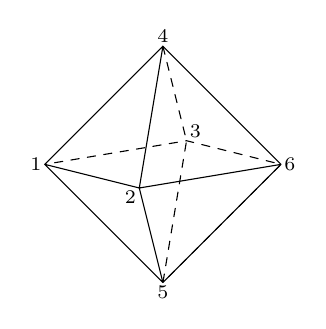
\begin{tikzpicture}[z={(-.2cm,-.2cm)},
			line join=round, line cap=round,
			every node/.style = {inner sep=1pt, font=\scriptsize}
			]
			\draw 
			(0,1.5,0) node[above] {$4$} --
			(-1.5,0,0) node[left] {$1$} --
			(0,-1.5,0) node[below] {$5$} --
			(1.5,0,0) node[right] {$6$} --
			(0,1.5,0) --
			(0,0,1.5) node[below left] {$2$} --
			(0,-1.5,0) --
			(1.5,0,0) -- 
			(0,0,1.5) -- 
			(-1.5,0,0);
			\draw[dashed] 
			(0,1.5,0) -- 
			(0,0,-1.5) node[above right] {$3$} -- 
			(0,-1.5,0) --
			(1.5,0,0) -- 
			(0,0,-1.5) -- 
			(-1.5,0,0);
			\end{tikzpicture} 
			
			\begin{itemize}
				\item[$t_1$:] 
				$1 + \frac{1}{4}(t_2+t_3+t_4+t_5)$
				\item[$t_2$ and $t_3$:] 
				$1 + \frac{1}{4}(t_1+t_4+t_5+t_6)$
				\item[$t_4$ and $t_5$:] 
				$1 + \frac{1}{4}(t_1+t_2+t_3+t_6)$
				\item[$t_6$:] 
				$0$
			\end{itemize}
		
			Due to symmetry, we can further state that $t_2=t_3=t_4=t_5$. Therefore:
			
			\[ t_1=1+\frac{1}{4}(4t_2)=1+t_2 \]
			\[ t_2=1+\frac{1}{4}(t_1+2t_2+0)=1+\frac{1}{4}t_1+\frac{1}{2}t_2\Rightarrow t_2=2+\frac{1}{2}t_1 \]
			\[ t_1=1+2+\frac{1}{2}t_1\Rightarrow \frac{1}{2}t_1=3\therefore \mybox{$t_1=6$ minutes}\]
			
			\item[(b)] Compute the same expected value if the octahedron is replaced by a cube (where $A$ and $B$ are still opposite vertices).
			
			\subparagraph{Solution} Let $t_i$ be the expected amount of time for the ant to reach vertex 8 from vertex $i$ on the cube.
			
			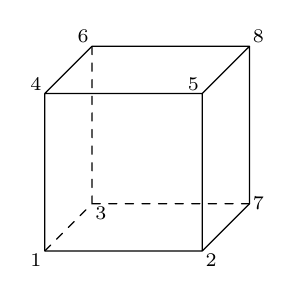
\begin{tikzpicture}[z={(-.3cm,-.3cm)},
			line join=round, line cap=round,
			every node/.style = {inner sep=1pt, font=\scriptsize}
			]
			\draw 
			(0,2,0) node[above left] {$4$} --
			(0,0,0) node[below left] {$1$} --
			(2,0,0) node [below right] {$2$} --
			(2,2,0) node[above left] {$5$} --
			(0,2,0) --
			(0,2,-2) node[above left] {$6$} --
			(2,2,-2) node[above right] {$8$} --
			(2,0,-2) node[right] {$7$}
			(2,2,-2) --
			(2,2,0)
			(2,0,0) --
			(2,0,-2);
			\draw[dashed] 
			(0,0,0) --
			(0,0,-2) node[below right] {$3$} --
			(0,2,-2)
			(0,0,-2) --
			(2,0,-2);
			\end{tikzpicture} 
			
			\begin{itemize}
				\item[$t_1$:] 
				$1 + \frac{1}{3}(t_2+t_3+t_4)$
				\item[$t_2$:] 
				$1 + \frac{1}{3}(t_1+t_5+t_7)$
				\item[$t_3$:] 
				$1 + \frac{1}{3}(t_1+t_6+t_7)$
				\item[$t_4$:] 
				$1 + \frac{1}{3}(t_1+t_5+t_6)$
				\item[$t_5$:] 
				$1 + \frac{1}{3}(t_2+t_4+t_8)$
				\item[$t_6$:] 
				$1 + \frac{1}{3}(t_3+t_4+t_8)$
				\item[$t_7$:] 
				$1 + \frac{1}{3}(t_2+t_3+t_8)$
				\item[$t_8$:] 
				$0$
			\end{itemize}
		
			Due to symmetry, we can further state that $t_2=t_3=t_4$ and $t_5=t_5=t_7$. Therefore:
			\[ t_1=1+\frac{1}{3}(3t_2)=1+t_2 \]
			\[ t_2=1+\frac{1}{3}(t_1+2t_3) \]
			\[ t_5=1+\frac{1}{3}(2t_2+0)=1+\frac{2}{3}(t_2) \]
			\[ t_2=1+\frac{1}{3}(t_1+2(1+\frac{2}{3}t_2))=1+\frac{1}{3}(t_1+2+\frac{4}{3}t_2)=1+\frac{1}{3}t_1+\frac{2}{3}+\frac{4}{9}t_2\Rightarrow \]
			\[ \frac{5}{9}t_2=1+\frac{1}{3}t_1+\frac{2}{3}\Rightarrow t_2=\frac{15+3t_1}{5} \]
			\[ t_1=1+\frac{15+3t_1}{5}\Rightarrow 5t_1=5+15+3t_1\Rightarrow 2t_1=20\therefore \mybox{$t_1=10$ minutes} \]
		\end{enumerate}
	
		\item[\textbf{Problem G4.}] For a positive integer $n$, let $f(n)$ denote the smallest positive integer which neither divides $n$ nor $n+1$.
		
		\begin{enumerate}
			\item[(a)] Find the smallest $n$ for which $f(n)=9$.
			
			\subparagraph{Solution} Since $f(n)=9$, all integers from 1 to 8 must be factors of $n$ or $n+1$. Furthermore, since 8 is a multiple of both 4 and 2, and 6 is a multiple of 2, we can narrow down the necessary factors to 3, 5, 7, and 8. Therefore, either $n$ or $n+1$ must end in a 0 or 5. Combining this limitation with the fact that either $n$ or $n+1$ must be a multiple or one away from a multiple of 3, 7, or 8 further narrows down the possibilities. Using this method, the clear answer reveals itself as \mybox{$n=104$}, since the factors of 104 and 105 are 3, 5, 8, and 13.
			
			\item[(b)] Is there an $n$ for which $f(n)=2018$?
			
			\subparagraph{Solution} Similar to (a), all integers from 1 to 2017 must be factors of $n$ or $n+1$. However, since the two factors of 2018 (2 and 1009) both fall into that range, the answer cannot simply be 2017!. Therefore, and equation can be setup to find a number pair where 1009 is only a factor of one of the numbers:
			\[ \frac{2017!}{1009}=1009x+1\Rightarrow 1009^2x=2017!-1009\Rightarrow x=\frac{2017!-1009}{1009^2} \]
			Plugging the above expression into SageMath and checking if it is an integer returns true, meaning \mybox{$n=\frac{2017!-1009}{1009}$}.
			
			\item[(c)] Which values can $f(n)$ take as $n$ varies?
			
			\subparagraph{Solution} $f(n)$ is always the smallest positive integer which cannot be found in the prime factorization of either $n$ or $n+1$.
		\end{enumerate}
	
		\item[\textbf{Problem G5.}] A pile with $n>=3$ stones is given. Two players Alice and Bob alternate taking stones, with Alice moving first. On a turn, if there are $m$ stones left, a player loses if $m$ is prime; otherwise he/she may pick a divisor $d | m$ such that $1<d<m$ and remove $d$ stones from the pile.
		
		\begin{enumerate}
			\item[(a)] Which player wins for $n=6$, $n=8$, $n=10$?
			
			\item[(b)] Determine the winning player of all $n$.
		\end{enumerate}
	
		\item[\textbf{Problem G6.}] A perfect power is an integer of the form $b^n$, where $b$, $n>=2$ are integers. Consider matrices $2\times2$ whose entries are perfect powers; we call such matrices \textit{good}.
		
		\begin{enumerate}
			\item[(a)] Find an example fo a good matrix with determinant 2019.
			
			\item[(b)] Do there exists any such matrices with determinant 1? If so, comment on how many there could be. (Possible hint: use the theory of Pell equations.)
		\end{enumerate}
	
		\item[\textbf{Problem G7.}] We consider a fixed triangle $ABC$ with side lengths $a=BC,b=CA,c=AB$, and a variable point $X$ in the interior. The lines through $X$ parallel to $\overline{AB}$ and $\overline{AC}$, together with line $\overline{BC}$, determine a triangle $T_a$. The triangles $T_b$ and $T_c$ are defined in a similar way, as shown in the figure. Let $S$ and $p$ denote the average area and perimeter, respectively, of the three triangles $T_a,T_b,T_c$.
		
		\begin{enumerate}
			\item[(a)] Determine all possible values of $S$ as $X$ varies, in terms of $a,b,c$.
			
			\item[(b)] Determine all possible values of $p$ as $X$ varies, in terms of $a,b,c$.
		\end{enumerate}
	\end{itemize}
\end{document}